\section{KẾT QUẢ THỰC HIỆN}
\subsection{Kết quả thiết kế phần cứng qua Altium}
\begin{figure}[h!]
    \centering
    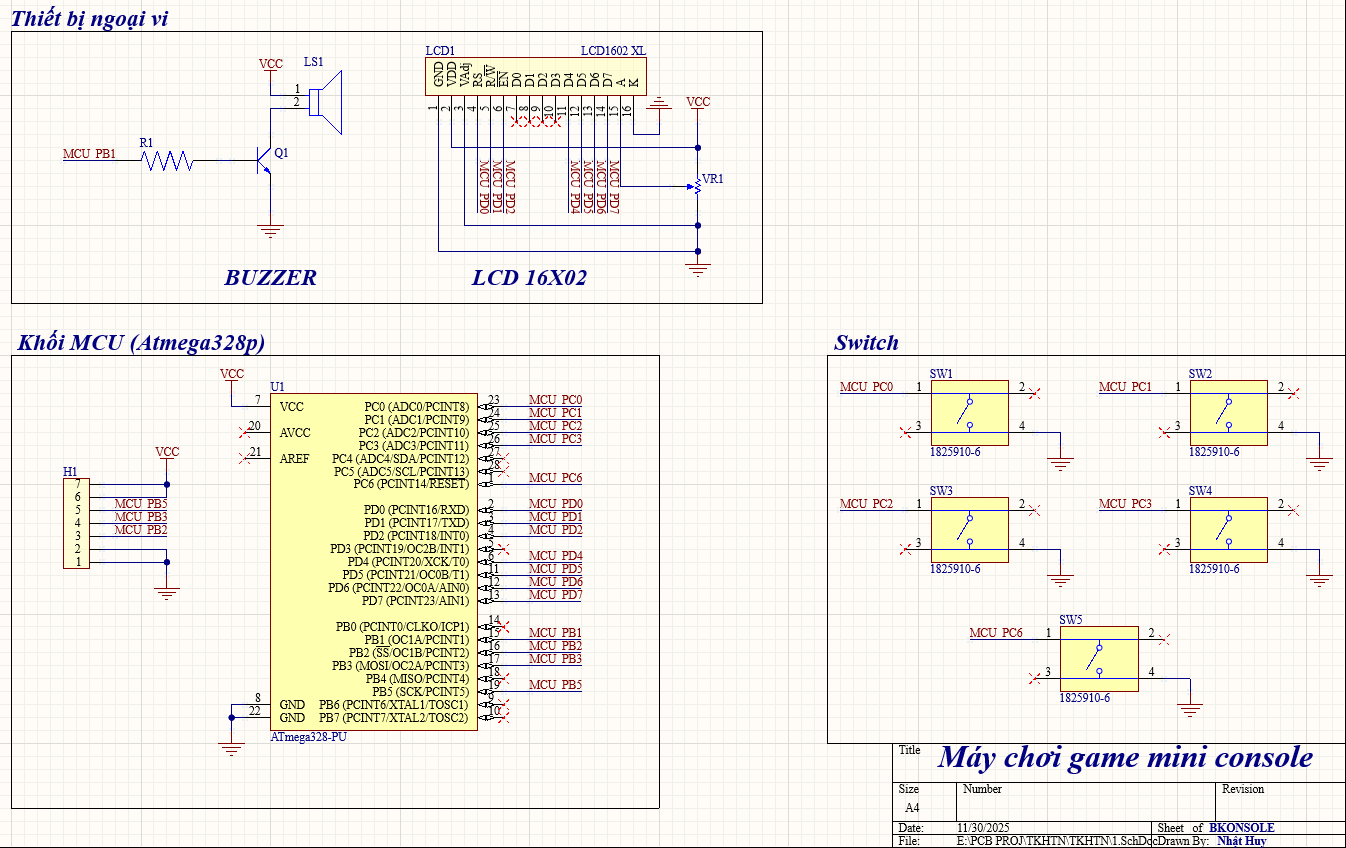
\includegraphics[width=0.85\textwidth]{img/SCHEM_main.png}
    \caption{Mạch nguyên lý của hệ thống}
\end{figure}
\subsection{Kết quả mô phỏng phần cứng qua Altium}
\begin{figure}[h!]
    \centering
    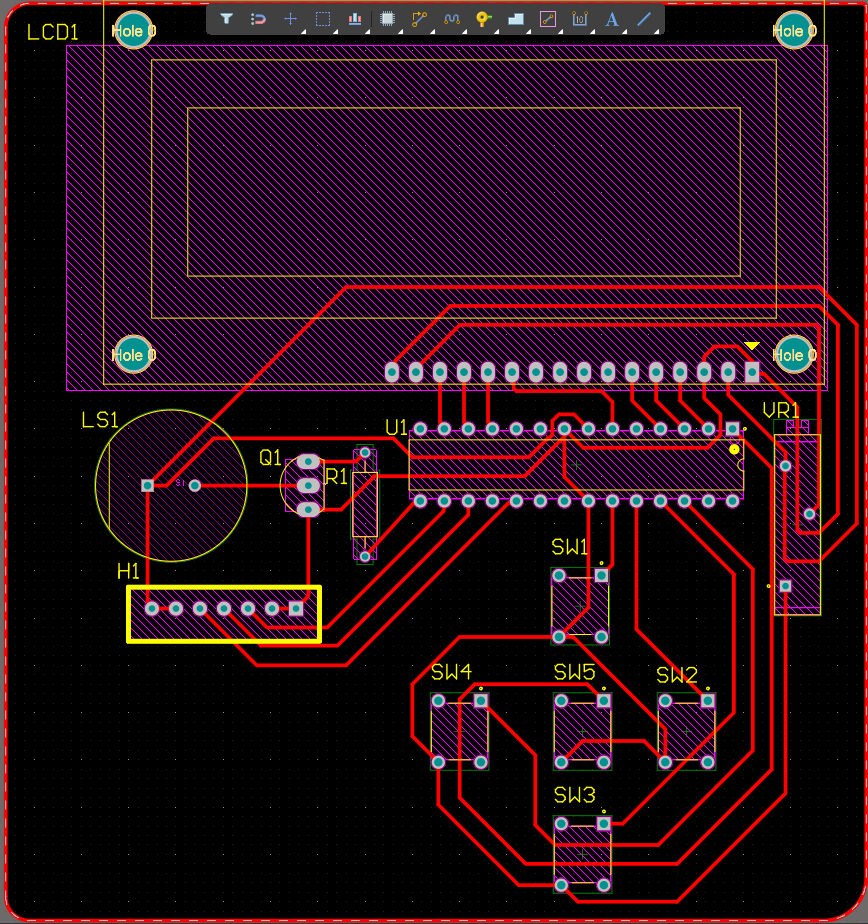
\includegraphics[width=0.5\textwidth]{img/SCHEM_2D.png}
    \caption{Mạch in 2D của hệ thống}
\end{figure}

\begin{figure}[h!]
    \centering
    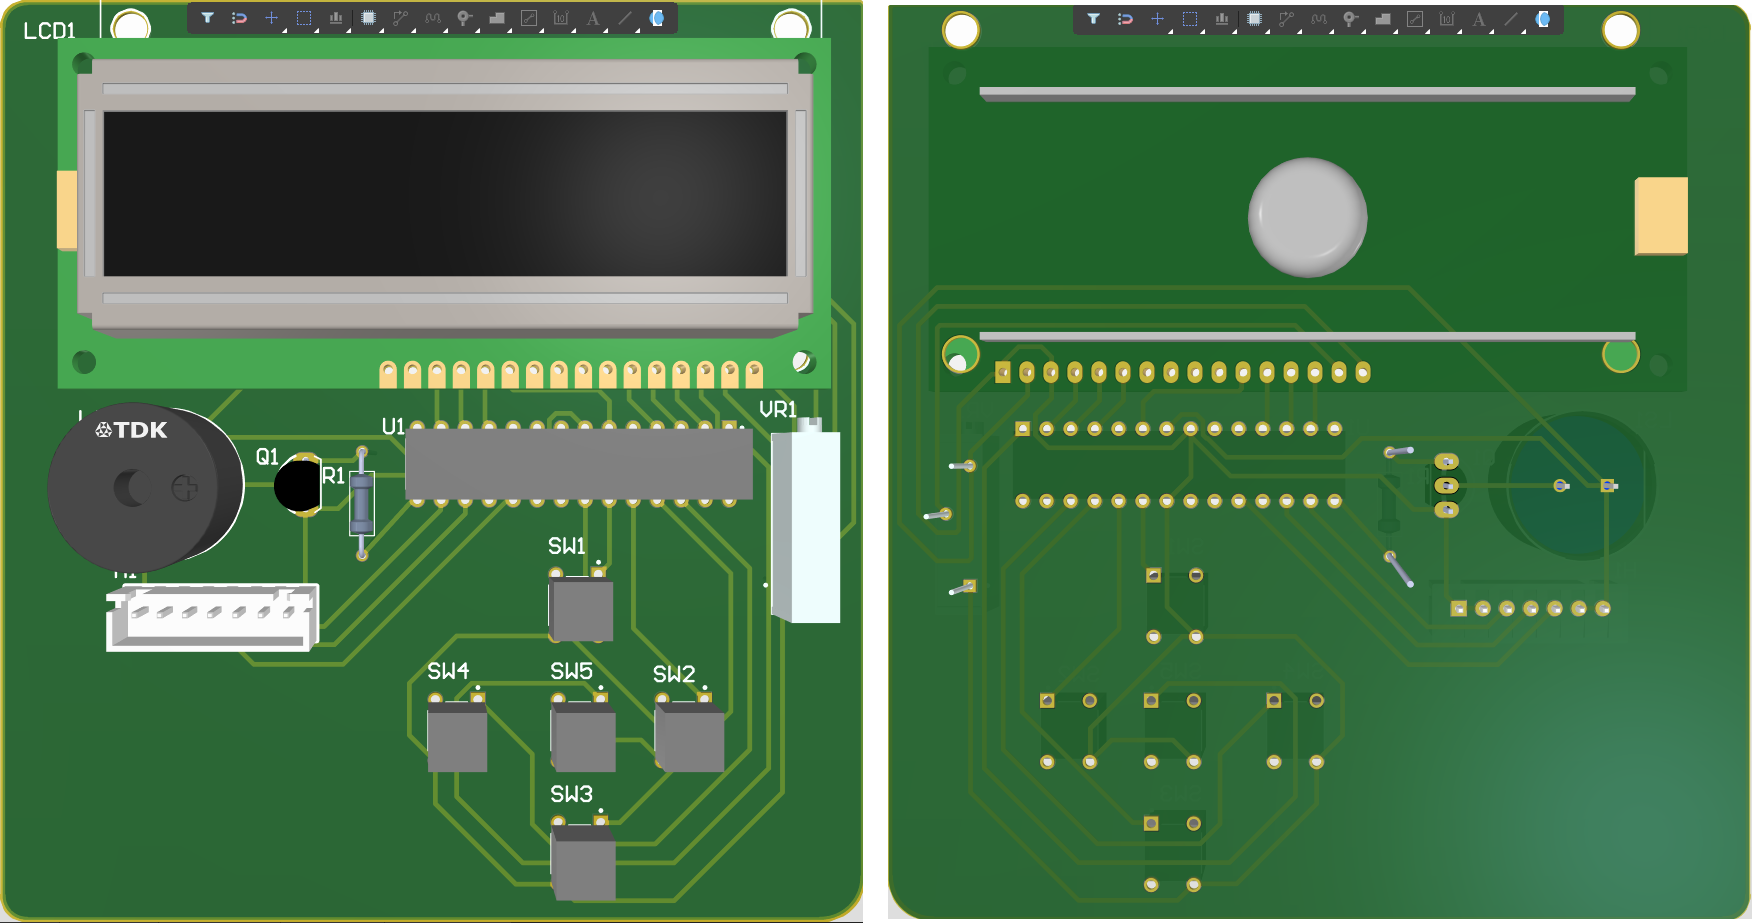
\includegraphics[width=.9\textwidth]{img/SCHEM_3D.png}
    \caption{Mạch in 3D (trước và sau) của hệ thống}
\end{figure}
\subsection{Kết quả mô phỏng Proteus}
\begin{figure}[h!]
    \centering
    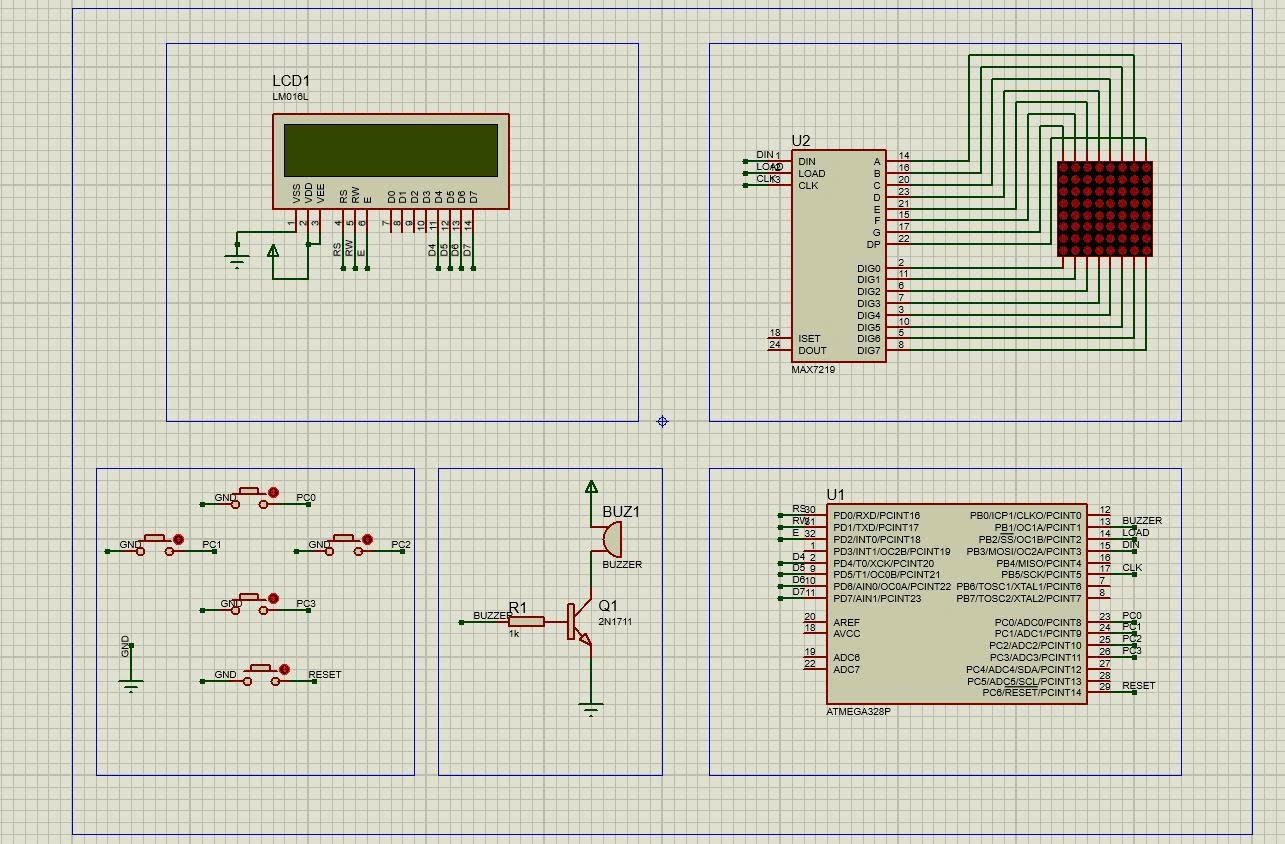
\includegraphics[width=.8\textwidth]{img/SCHEM_proteus.png}
    \caption{Mạch mô phỏng Proteus}
\end{figure}
\newpage
\subsection{Kết quả thực hiện phần cứng}
\begin{figure}[h!]
    \centering
    \includegraphics[width=.6\textwidth]{img/demo.png}
    \caption{Kết quả gia công phần cứng}
\end{figure}
\subsection{Kết quả chạy thực tế}
Mạch thực hiện đúng chức năng được đề ra và đính kèm video là chạy thử mạch.